\LectureAnswerSection\subsection*{两级提示}
\phantomsection\label{hint:at2:drill:1}
\LectureHint{at2:drill:1}{先算能量和角动量，不先猜端点。}{用径向加速度的符号检查近远地点。}
\phantomsection\label{hint:at2:drill:2}
\LectureHint{at2:drill:2}{由原角动量与点火后能量求精确参数。}{展开两端距离和周期，区分一阶与二阶变化。}
\phantomsection\label{hint:at2:drill:3}
\LectureHint{at2:drill:3}{同一余弦值对应两个不同象限。}{连续取偏近点角，时间差不能只相减主值。}
\phantomsection\label{hint:at2:drill:4}
\LectureHint{at2:drill:4}{先证明所选区间内导数为正。}{迭代后用残差除以导数下界检查误差。}
\phantomsection\label{hint:at2:drill:5}
\LectureHint{at2:drill:5}{先由真近点角求半径。}{再由半径恢复偏近点角，并按去程选正弦符号。}
\phantomsection\label{hint:at2:drill:6}
\LectureHint{at2:drill:6}{先平均速度平方，不能先平均速度再平方。}{用瞬时公式检验逐点等式的成立位置。}
\phantomsection\label{hint:at2:drill:7}
\LectureHint{at2:drill:7}{逐次代入时保留小参数的阶数。}{真近点角的一阶修正需要合并两项修正。}
\phantomsection\label{hint:at2:drill:8}
\LectureHint{at2:drill:8}{先由周期律确定保持不变的参数。}{再逐项比较，区分瞬时量和时间平均量。}
\Needspace{8\baselineskip}\subsection*{详解}
\begin{drillsolution}{at2:drill:1}
图\ref{fig:at2:drill:1:s} 初态无径向速度，但切向速度大于当地圆轨道速度。先算 $\varepsilon=3\mu/(4r_0)-\mu/r_0=-\mu/(4r_0)$、$h^2=3\mu r_0/2$。
\typeout{ASTROFIG:fig:at2:drill:1:p}\fig{fig:at2:drill:1:p}{解答过程：由瞬时分量恢复轨道参数}{\begin{tikzpicture}[scale=.85]
\draw[world](-1.5,0)ellipse(3 and 2.598076);\fill(0,0)circle(2pt)node[below right]{$F$};\fill(1.5,0)circle(1.5pt)node[right]{$P$};\fill(-4.5,0)circle(1.5pt)node[left]{$A$};\draw[guide](-4.5,0)--(1.5,0);\node[below]at(-1.5,0){$O$};\node at(-1.5,1){$a=2r_0,\ e=1/2$};\node at(-1.5,-1){$r_p=r_0,\ r_a=3r_0$};
\end{tikzpicture}}

图\ref{fig:at2:drill:1:p} 给 $a=-\mu/(2\varepsilon)=2r_0$、$p=h^2/\mu=3r_0/2$，所以 $e=\sqrt{1-p/a}=1/2$。两端为 $r_p=a(1-e)=r_0$、$r_a=3r_0$，此点是近地点。周期 $T=2\pi\sqrt{8r_0^3/\mu}$。检验径向加速度 $\ddot r=v_t^2/r_0-\mu/r_0^2=\mu/(2r_0^2)>0$，从此点开始距离增大，与近地点判断一致。\end{drillsolution}
\begin{drillsolution}{at2:drill:2}
    图\ref{fig:at2:drill:2:s} 脉冲不改角动量，$h^2=\mu r_0$。令 $s=u/v_c$，能量 $\varepsilon=(u^2-v_c^2)/2$，所以
    \[a=\frac{r_0}{1-s^2},\quad p=r_0,\quad e=s,\quad
    r_p=\frac{r_0}{1+s},\quad r_a=\frac{r_0}{1-s}.
    \]
    \typeout{ASTROFIG:fig:at2:drill:2:p}\fig{fig:at2:drill:2:p}{解答过程：径向小脉冲的精确轨道与线性极限}{\begin{tikzpicture}[scale=.85]
\draw[world](-1.5,0)ellipse(3 and 2.598076);\fill(0,0)circle(2pt)node[below right]{$F$};\fill(1.5,0)circle(1.5pt)node[right]{$P$};\fill(-4.5,0)circle(1.5pt)node[left]{$A$};\draw[guide](-4.5,0)--(1.5,0);\node[below]at(-1.5,0){$O$};\node at(-1.5,1){$r_p=r_0/(1+s)$};\node at(-1.5,-1){$r_a=r_0/(1-s)$};
\end{tikzpicture}}

    图\ref{fig:at2:drill:2:p} 周期 $T=T_0(1-s^2)^{-3/2}=T_0[1+3s^2/2+O(s^4)]$，可见周期没有一阶变化。两端距离分别为 $r_0(1-s)+O(r_0s^2)$、$r_0(1+s)+O(r_0s^2)$，径向一阶振幅 $r_0s=u/n_0$。它与微积分专题用初值解得的 $\eta=(u/n_0)\sin n_0t$ 相符，而精确周期与上下极值的非对称属于更高阶效应。本题通过完整轨道参数检查线性模型，不再重复通用的一阶微分方程推导。\end{drillsolution}
\begin{drillsolution}{at2:drill:3}
图\ref{fig:at2:drill:3:s} 的两个位置是短轴端，去程 $E_1=\pi/2$，回程 $E_2=3\pi/2$。沿连续增大的 $E$ 代入时间差，
\[\Delta t=\frac{(3\pi/2+e)-(\pi/2-e)}n=\frac{\pi+2e}{n}.\]
\typeout{ASTROFIG:fig:at2:drill:3:p}\fig{fig:at2:drill:3:p}{解答过程：同一半径的去程与回程}{\begin{tikzpicture}[scale=.85]
\draw[world](-1.5,0)ellipse(3 and 2.598076);\fill(0,0)circle(2pt)node[below right]{$F$};\fill(1.5,0)circle(1.5pt)node[right]{$P$};\fill(-4.5,0)circle(1.5pt)node[left]{$A$};\draw[guide](-4.5,0)--(1.5,0);\node[below]at(-1.5,0){$O$};\fill(-1.5,2.598)circle(2pt);\fill(-1.5,-2.598)circle(2pt);\draw[flow](-2.4,2.35)--(-3,2);\draw[flow](-3,-2)--(-2.4,-2.35);
\end{tikzpicture}}

图\ref{fig:at2:drill:3:p} 这段运动经过远地点，所以时间大于半周期。两点的总速率均为 $\sqrt{\mu/a}$，切向分量均为 $h/a$，径向分量大小相同、符号相反。具体由 $\dot r=na e\sin E/(1-e\cos E)$ 得 $v_r=\pm nae$。两次经过相同半径不意味着两速度矢量相同，也不意味着两时刻相差恰好半周期。\end{drillsolution}
\begin{drillsolution}{at2:drill:4}
图\ref{fig:at2:drill:4:s} 需解 $F(E)=E-0.6\sin E-1=0$，导数 $F'=1-0.6\cos E\ge0.4$，故解唯一。由 $E=1+0.6\sin E$ 可先将正解夹在 $[1,1.6]$。
\typeout{ASTROFIG:fig:at2:drill:4:p}\fig{fig:at2:drill:4:p}{解答过程：开普勒方程的数值解}{\begin{tikzpicture}[scale=.85]
\draw[axis](-.2,0)--(4.5,0)node[right]{$E$};\draw[axis](0,-.2)--(0,2.4)node[above]{$F$};\draw[world,domain=1:2,samples=70]plot(\x,{\x-.6*sin(deg(\x))-1});\fill(1.6,0)circle(2pt)node[above]{$E\simeq1.600$};
\end{tikzpicture}}

按 图\ref{fig:at2:drill:4:p} 的曲线交点，用牛顿公式 $E_{k+1}=E_k-F(E_k)/F'(E_k)$。取 $E_0=1.6$，得到约 $1.599749$，下一次变化小于 $10^{-7}$，因此 $E\simeq1.600$。代回残差后，由中值定理 $|E-E_*|\le|F(E)|/0.4$，可把函数残差转成角度误差；只看到相邻两次显示相同小数，并不自动证明所需误差。\end{drillsolution}
\begin{drillsolution}{at2:drill:5}
  图\ref{fig:at2:drill:5:s} 此点 $r=p=a(1-e^2)$。由 $r=a(1-e\cos E)$，得 $\cos E=e$；去程取 $E=\arccos e$、$\sin E=\sqrt{1-e^2}$。
  \typeout{ASTROFIG:fig:at2:drill:5:p}\fig{fig:at2:drill:5:p}{解答过程：经过半通径位置的时间}{\begin{tikzpicture}[scale=.85]
\draw[world](-1.5,0)ellipse(3 and 2.598076);\fill(0,0)circle(2pt)node[below right]{$F$};\fill(1.5,0)circle(1.5pt)node[right]{$P$};\fill(-4.5,0)circle(1.5pt)node[left]{$A$};\draw[guide](-4.5,0)--(1.5,0);\node[below]at(-1.5,0){$O$};\draw[guide](0,0)--(0,2.25);\node at(-2,1){$E=\arccos e$};
\end{tikzpicture}}

  图\ref{fig:at2:drill:5:p} 时间为 $t=[\arccos e-e\sqrt{1-e^2}]/n$。注意 $f$ 为直角不意味着 $E$ 也是直角；当 $e>0$，此位置尚未到达短轴端。若 $e\to0$，两角都趋直角，时间恢复四分之一周期。这是图中“焦点处的直角”和“中心辅助圆的直角”必须分开的例子。\end{drillsolution}
\begin{drillsolution}{at2:drill:6}
  图\ref{fig:at2:drill:6:s} 的活力式给 $\langle v^2\rangle=\mu(2\langle1/r\rangle-1/a)=\mu/a$，因此 $\langle K\rangle=\mu m/(2a)$，$\langle U\rangle=-\mu m/a$。
  \typeout{ASTROFIG:fig:at2:drill:6:p}\fig{fig:at2:drill:6:p}{解答过程：椭圆的平均动能与势能}{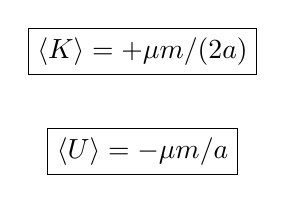
\begin{tikzpicture}[scale=.85]
\node[draw]at(0,1){$\langle K\rangle=+\mu m/(2a)$};\node[draw]at(0,-.5){$\langle U\rangle=-\mu m/a$};
\end{tikzpicture}}

  图\ref{fig:at2:drill:6:p} 所以 $2\langle K\rangle+\langle U\rangle=0$，而 $\langle K+U\rangle=-\mu m/(2a)$ 与每时刻总能量相同。若要求逐点 $2K+U=0$，代入 $K=\mu m(1/r-1/(2a))$ 得 $r=a$，仅在椭圆两个短轴端瞬时成立；圆轨道才处处成立。平均恒等式不能当作椭圆每一点的速度公式。\end{drillsolution}
\begin{drillsolution}{at2:drill:7}
  图\ref{fig:at2:drill:7:s} 从 $E=M+e\sin E$ 出发，在乘 $e$ 的项中用零阶 $E=M$，得 $E=M+e\sin M+O(e^2)$。
  \typeout{ASTROFIG:fig:at2:drill:7:p}\fig{fig:at2:drill:7:p}{解答过程：近圆轨道的一阶位置修正}{\begin{tikzpicture}[scale=.85]
\draw[axis](-.2,0)--(6.6,0)node[right]{$M$};\draw[axis](0,-.2)--(0,2.5)node[above]{$f-M$};\draw[world,domain=0:6.283,samples=100]plot(\x,{1.5*sin(deg(\x))});\node at(3,2){$f-M\simeq2e\sin M$};
\end{tikzpicture}}

  图\ref{fig:at2:drill:7:p} 再用 $f=E+e\sin E+O(e^2)$，得到 $f=M+2e\sin M+O(e^2)$；半径 $r=a(1-e\cos M)+O(ae^2)$。直接令 $f=M$ 的最大一阶误差为 $2e$ 弧度，出现在 $M=\pi/2,3\pi/2$ 附近。两处只是首阶最差位置，精确极值可有高阶偏移。计算近似时将零阶值代进已乘小参数的项，是因为产生的额外误差只有二阶。\end{drillsolution}
\begin{drillsolution}{at2:drill:8}
  图\ref{fig:at2:drill:8:s} 周期相同且中心参数相同，由 $T^2=4\pi^2a^3/\mu$ 得半长轴相同。近日点速度 $v_p=\sqrt{\mu/a}\sqrt{(1+e)/(1-e)}$ 随 $e$ 增大而增大，故第二颗更快。
  \typeout{ASTROFIG:fig:at2:drill:8:p}\fig{fig:at2:drill:8:p}{解答过程：同周期椭圆的近点速度比较}{\begin{tikzpicture}[scale=.85]
\node[draw]at(0,1){同 $T\Rightarrow$ 同 $a$};\node[draw]at(0,-.5){大 $e$：近点更快，面积更小};
\end{tikzpicture}}

  图\ref{fig:at2:drill:8:p} 平均动能都为 $\mu m/(2a)$，若两质量不同应比较单位质量平均动能；全周面积 $\pi a^2\sqrt{1-e^2}$ 随 $e$ 增大而减小，面积速度也同比减小，二者相除仍给相同周期。不能由周期相同推出角动量、轨道面积或瞬时速率均相同。\end{drillsolution}
